\chapter{TP 3 : Afficheurs 7 segments, MATLAB/Simulink et Asservissement}
\minitoc
\newpage

\section{Utilisation des afficheurs 7 segments}
Un afficheur 7 segments permet de représenter des chiffres décimaux en allumant des segments spécifiques (constitués de LED internes).
Pour cela, nous utiliserons la bibliothèque \textbf{SevSeg}, qui simplifie grandement l'affichage des chiffres sur l'afficheur sept segments en évitant d'avoir recours à de multiples instructions \texttt{digitalWrite()}. 

\paragraph{a) Affichage du nombre 5 avec un afficheur simple}
Dans un premier temps, nous réalisons le câblage d'un seul afficheur 7 segments pour afficher le chiffre 5.

\begin{figure}[H]
	\centering
	\begin{minipage}{0.48\textwidth}
		\centering
		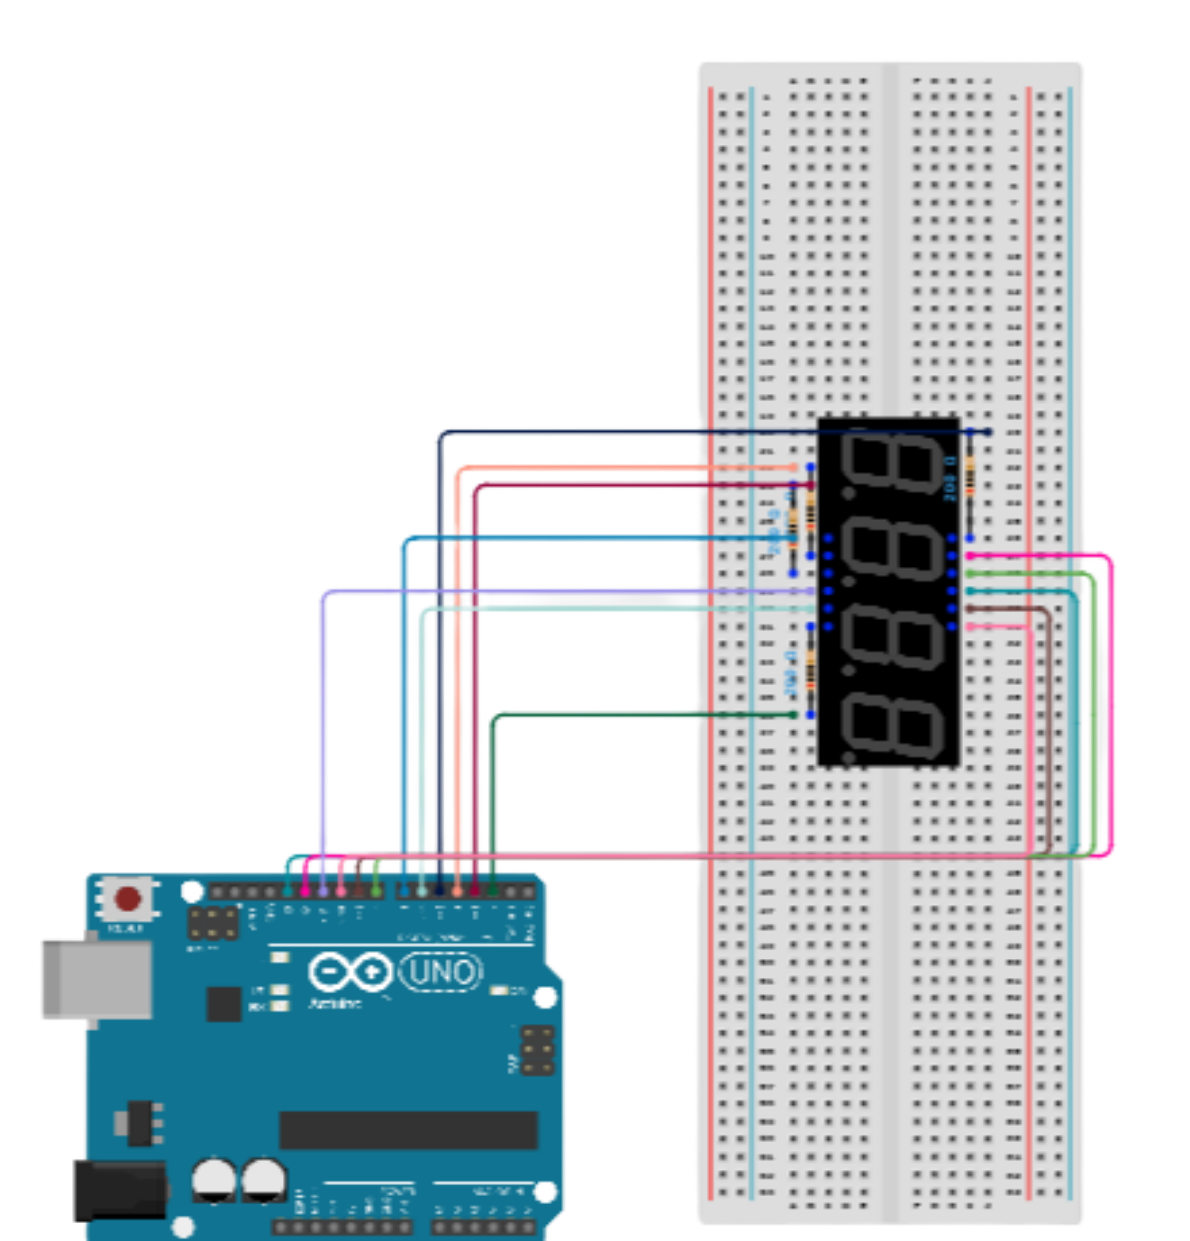
\includegraphics[width=\linewidth]{Image/3.Schema_Manip_a}
		\caption{Schéma du montage pour afficher le chiffre 5}
		\label{fig:schema_7seg_5}
	\end{minipage}\hfill
	\begin{minipage}{0.48\textwidth}
		\centering
		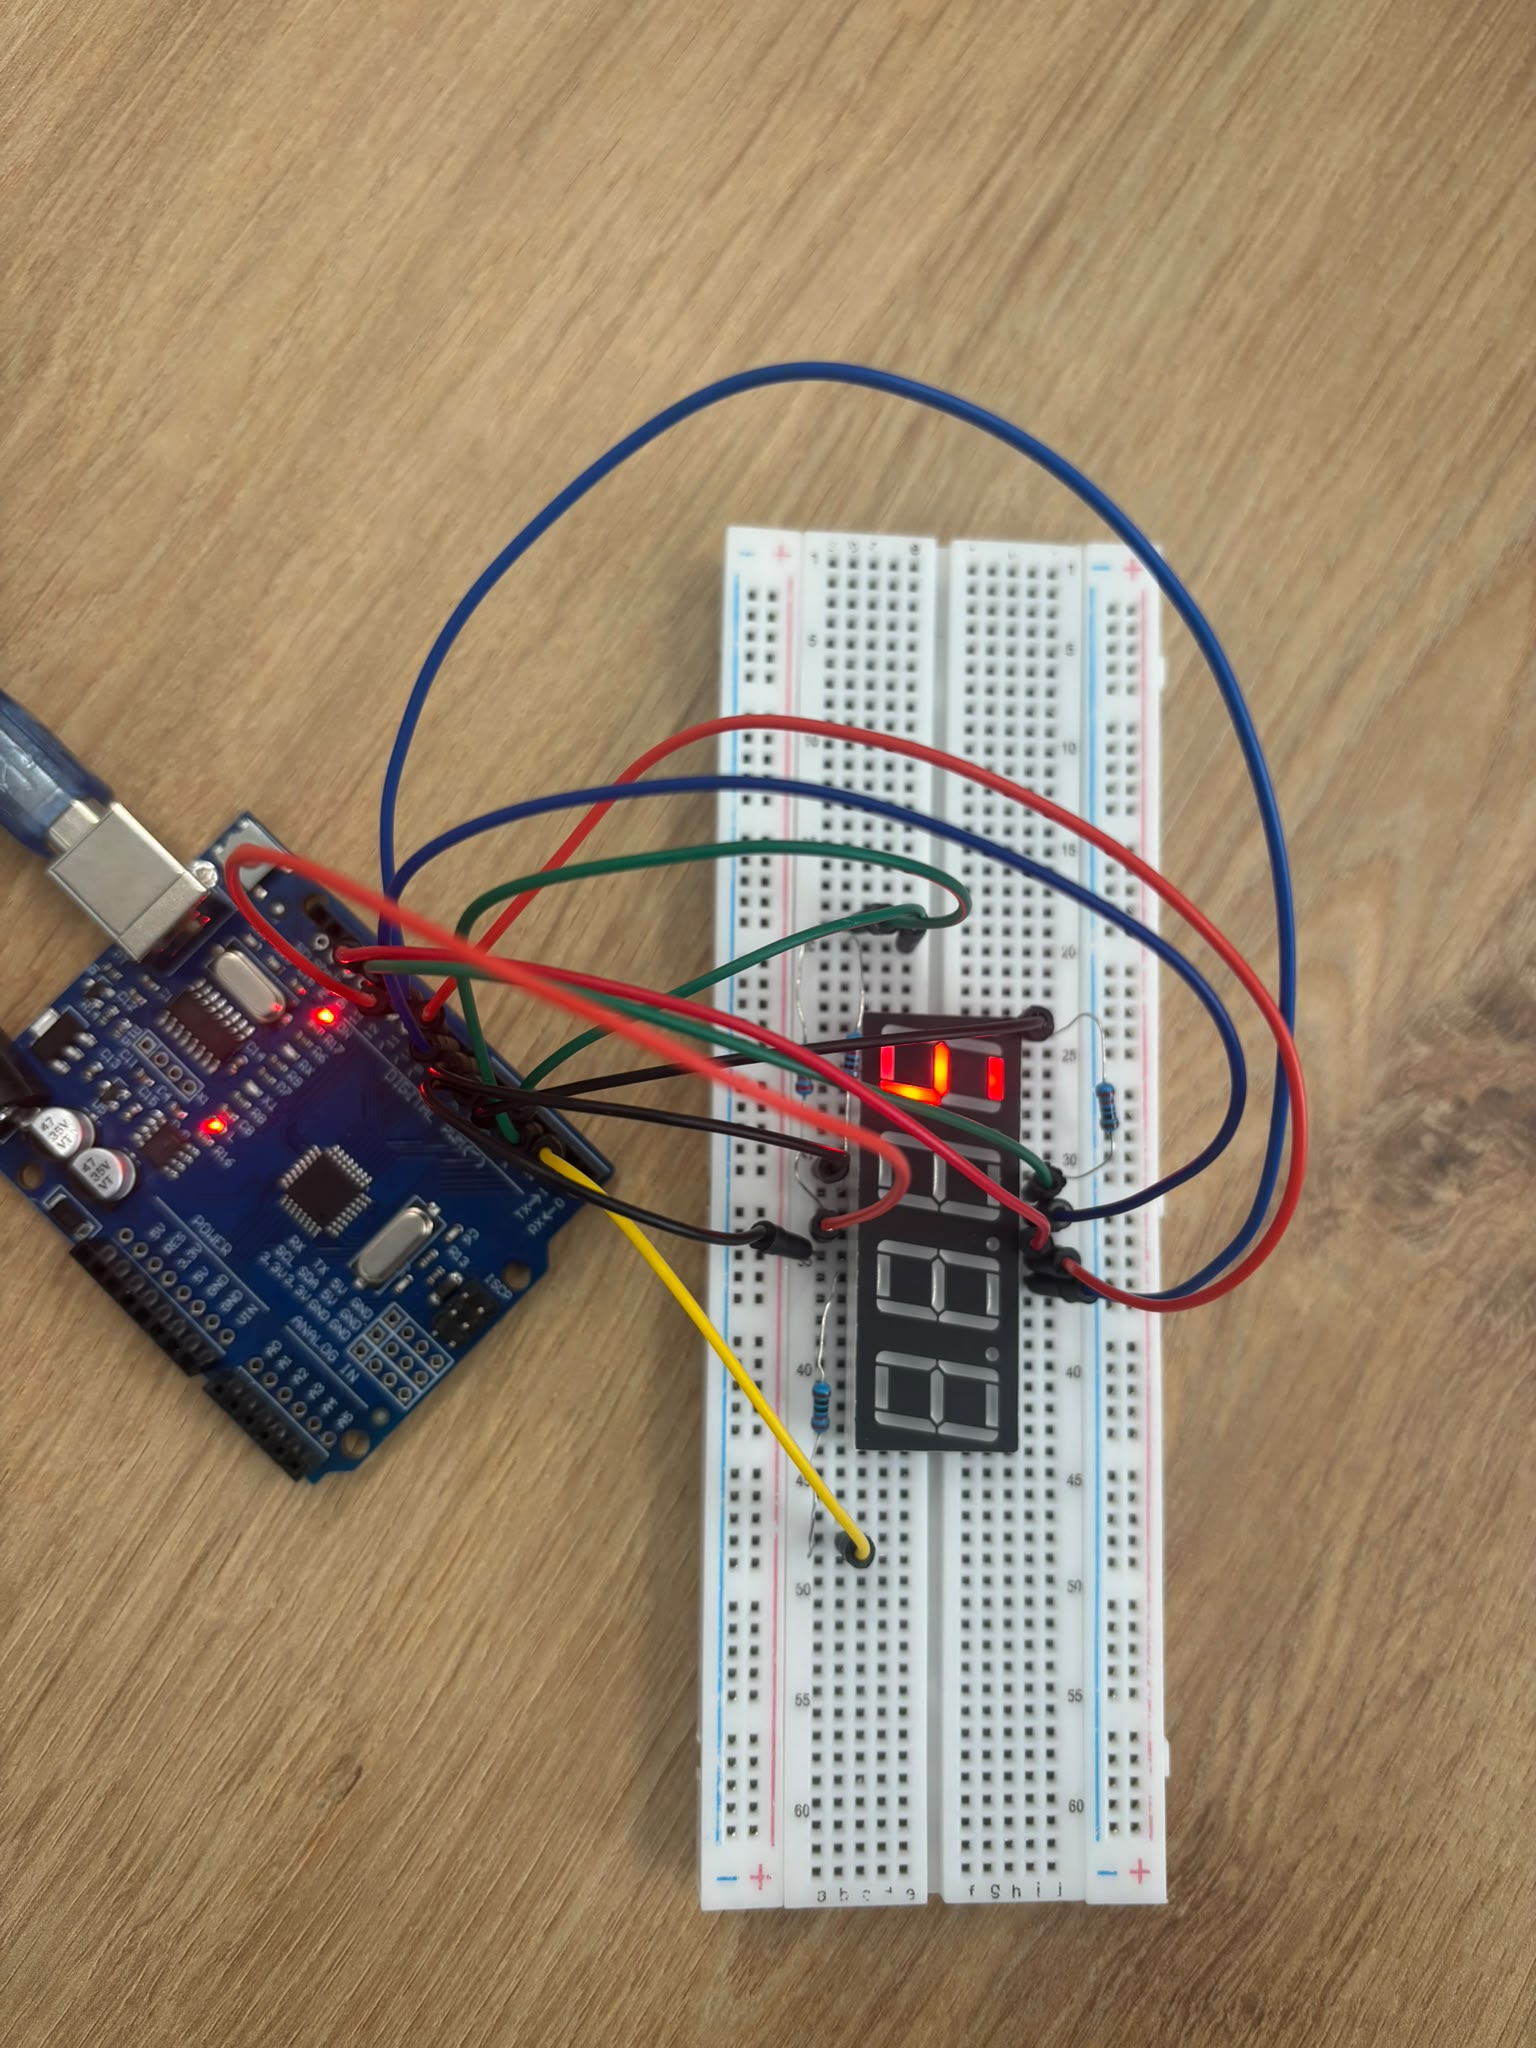
\includegraphics[width=\linewidth]{Image/3.Photo_Manip_a}
		\caption{Photo du montage de l'afficheur}
		\label{fig:photo_7seg_5}
	\end{minipage}
\end{figure}

\begin{lstlisting}
#include "SevSeg.h"

SevSeg sevseg; // Instancier un objet controleur a sept segments

int cap = A0;  // Broche analogique connectee au potentiometre
int val;       // Variable pour lire la valeur de la broche analogique

void setup() {
	byte numDigits = 4;
	byte digitPins[] = { 2, 3, 4, 5 };
	byte segmentPins[] = { 6, 7, 8, 9, 10, 11, 12, 13 };
	bool resistorsOnSegments = false;      // 'false' : les resistances sont sur les broches de chiffres
	byte hardwareConfig = COMMON_CATHODE;  // Voir README.md pour les options
	bool updateWithDelays = false;         // Recommande par defaut
	bool leadingZeros = false;             // 'true' pour afficher les zeros non significatifs
	bool disableDecPoint = true;           // 'true' si le point decimal n'est pas connecte
	
	sevseg.begin(hardwareConfig, numDigits, digitPins, segmentPins, resistorsOnSegments,
	updateWithDelays, leadingZeros, disableDecPoint);
	sevseg.setBrightness(100);
}

void loop() {
	val = analogRead(cap);    // Lecture du potentiometre (0 a 1023)
	sevseg.setNumber(val, 0); // Affiche la valeur lue (remplace le 5 fixe)
	sevseg.refreshDisplay();  // Doit tourner en continu sans delay()
}
\end{lstlisting}

\textbf{Observations :}L'afficheur s'allume correctement et forme le chiffre 5.

\paragraph{b) Affichage du nombre 25 et contrôle d'une LED en fonction de la température}
Nous combinons ici l'utilisation de deux afficheurs 7 segments pour afficher le nombre 25, tout en intégrant un capteur de température (comme le LM35 étudié au TP précédent). Une LED s'allume si la température dépasse 25 °C.

\begin{figure}[H]
	\centering
	\begin{minipage}{0.48\textwidth}
		\centering
		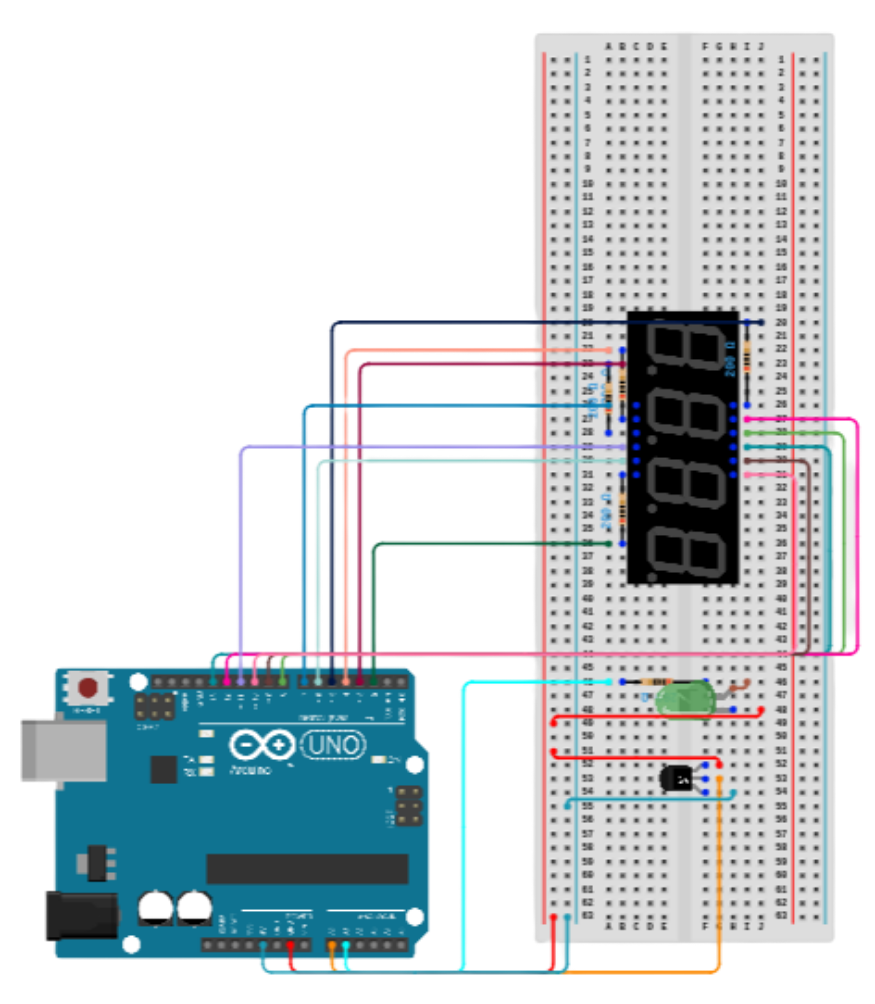
\includegraphics[width=\linewidth]{Image/3.Schema_Manip_b}
		\caption{Schéma du montage (Afficheurs + Capteur + LED)}
		\label{fig:schema_7seg_25}
	\end{minipage}\hfill
	\begin{minipage}{0.48\textwidth}
		\centering
		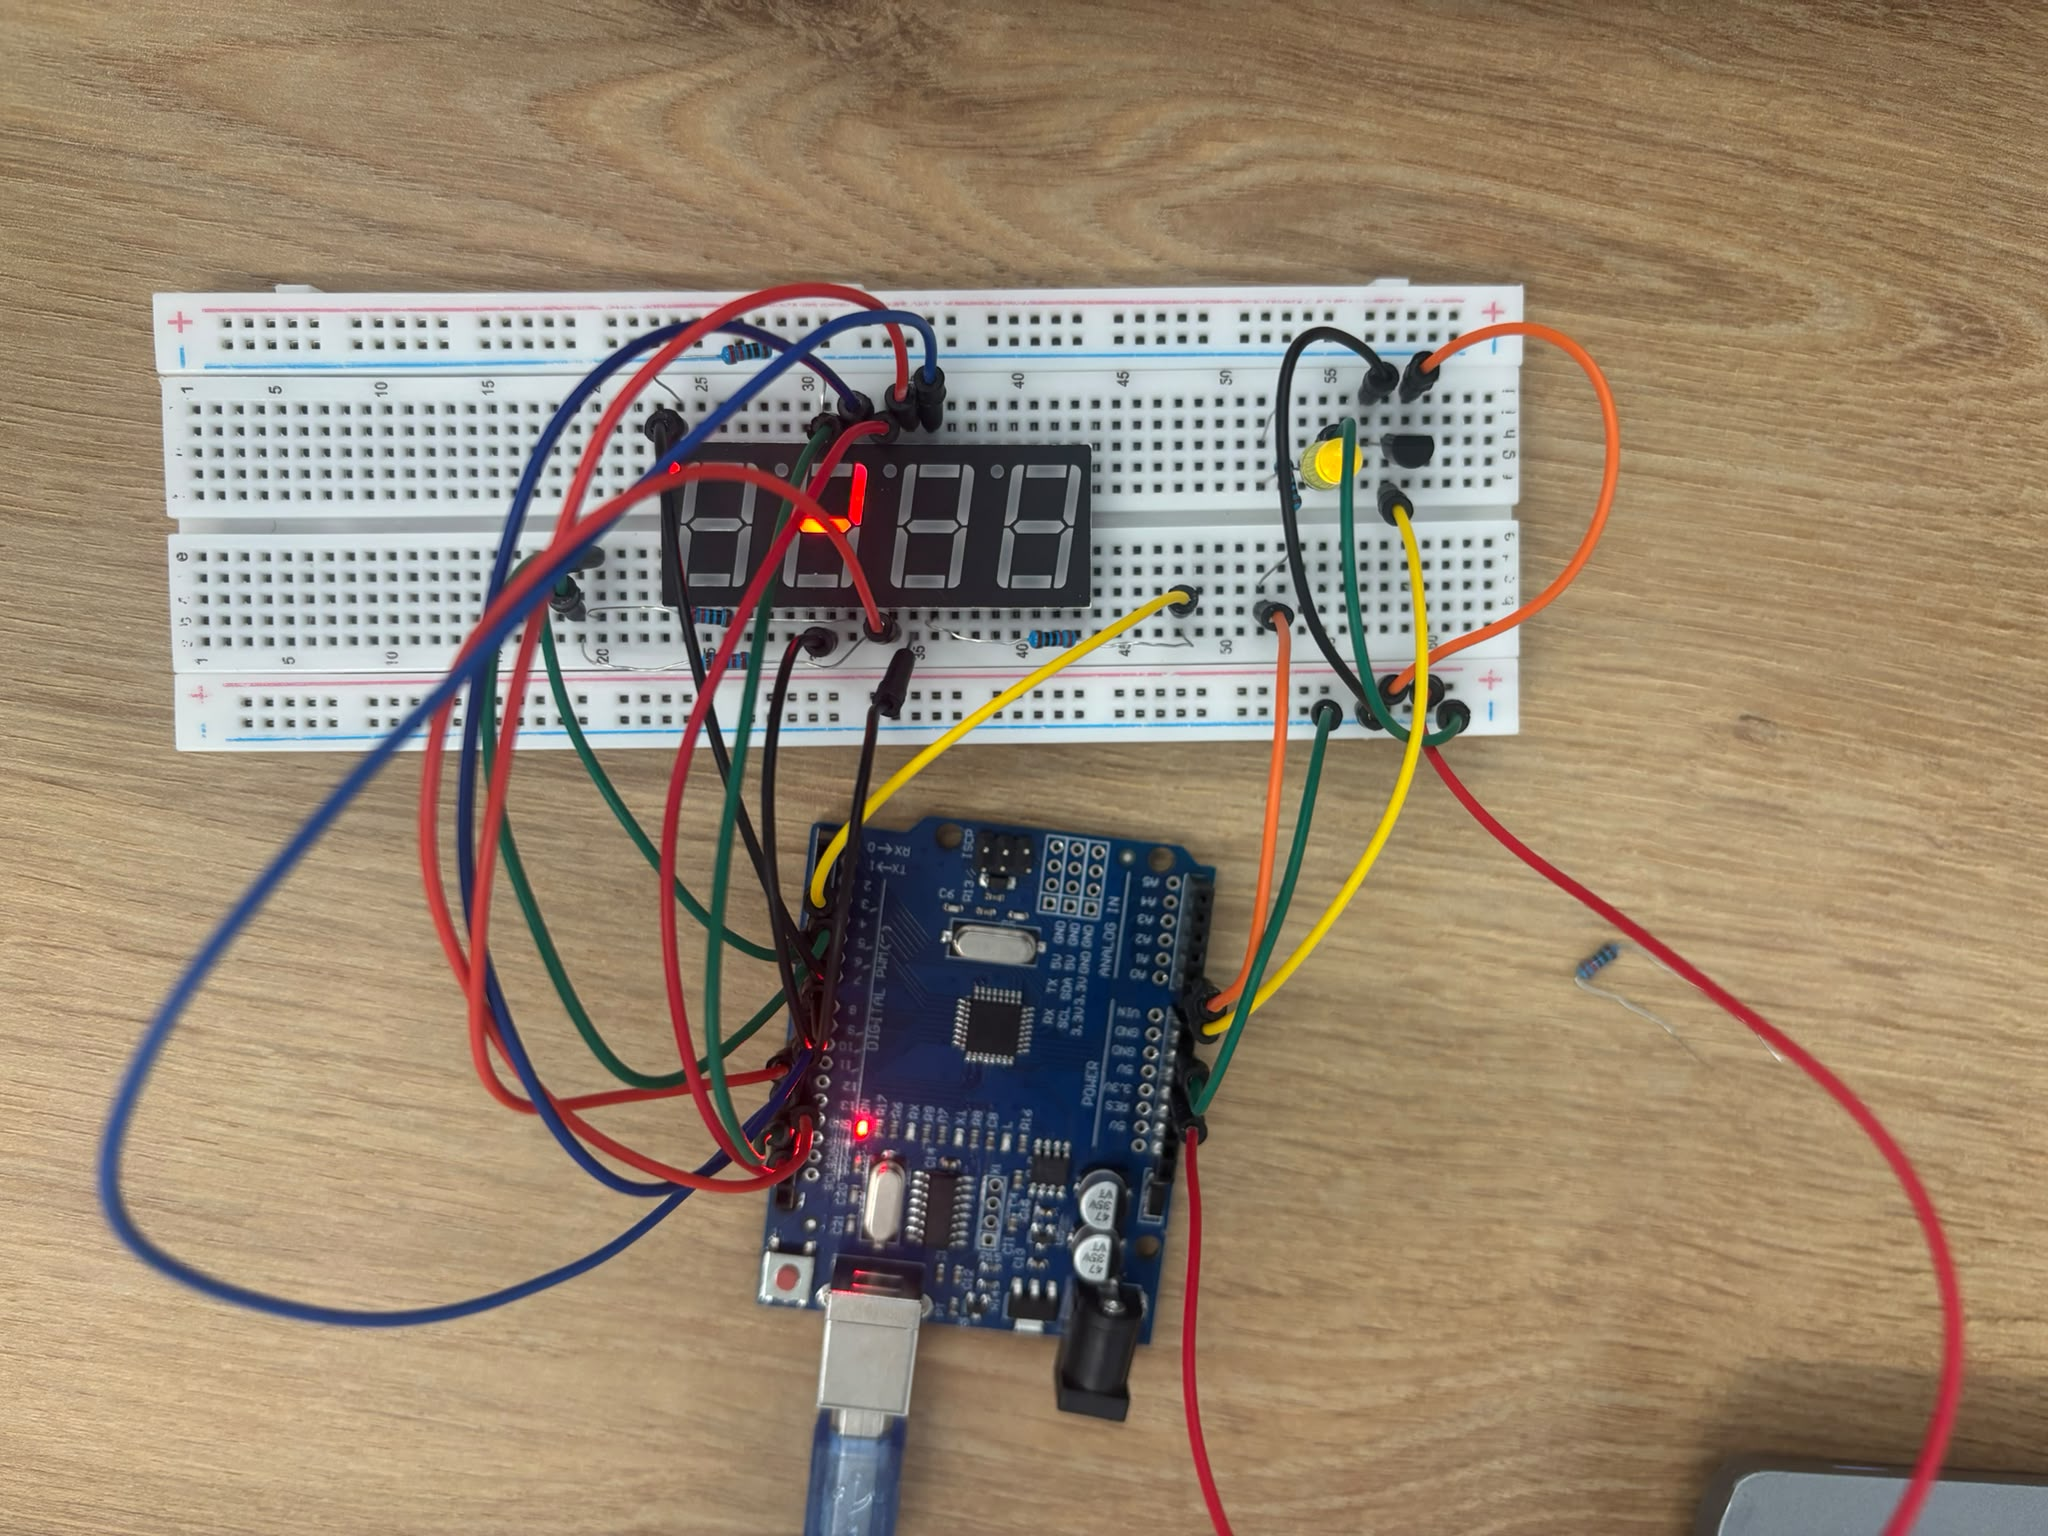
\includegraphics[width=\linewidth]{Image/3.Photo_Manip_b}
		\caption{Photo du montage (Afficheurs + Capteur + LED)}
		\label{fig:photo_7seg_25}
	\end{minipage}
\end{figure}

\begin{lstlisting}
	void loop() {
		val = analogRead(cap);
		
		float voltage = val * (5.0 / 1023.0) ;
		float temperature = voltage * 100.0; // 10 mV par C donc T = tension * 100
		if (temperature > 15) {
			digitalWrite(15, HIGH);
		} else {
			digitalWrite(15, LOW);
		}
		sevseg.setNumber(temperature, 0);
		sevseg.refreshDisplay();  // Doit etre execute a plusieurs reprises
	}
	
\end{lstlisting}

\textbf{Observations :} l'afficheur sept segment montre bien la valeur perçu par le capteur de température et la LED s'allume quand l'afficher affiche une valeur supérieur a 15 comme indiqué dans notre programme.

\paragraph{c) Compteur de 1 à 99 avec deux afficheurs 7 segments}
Nous programmons ensuite la carte pour incrémenter et afficher automatiquement les nombres de 1 à 99 en utilisant nos deux afficheurs 7 segments. Nous allons juste changer le programme et pas la partie montage car elle est déjà fonctionnelle

\begin{lstlisting}
	void loop() {
		
		for (int i =0 ; i<100 ; i++){ // notre boucle for pour afficher de 0 a 99
			sevseg.setNumber(i, 0);
			
			sevseg.refreshDisplay(); 
			delay(1000);
			
		};
		delay(1000);
	}
	
\end{lstlisting}

\textbf{Observations :} Nous observons bien le compteur fonctionner du chiffre 1 au nombre 99.

\section{Interfaçage Arduino et MATLAB/Simulink}
L'environnement Simulink permet de commander la carte Arduino en utilisant des blocs graphiques de la librairie "Simulink Support Package for Arduino Hardware".

\paragraph{d) Commande d'une LED depuis MATLAB/Simulink}
Nous réalisons un programme Matlab 

\begin{figure}[H]
	\centering
	% \includegraphics[width=0.7\linewidth]{Image/3.Simulink_LED}
	\caption{Modèle Simulink pour la commande de la LED}
	\label{fig:simulink_led}
\end{figure}

\begin{lstlisting}
	clear a;
	a = arduino('/dev/ttyUSB0', 'Uno');
	
	writeDigitalPin(a, 'D13', 1);
\end{lstlisting}
\begin{figure}[H]
	\centering
	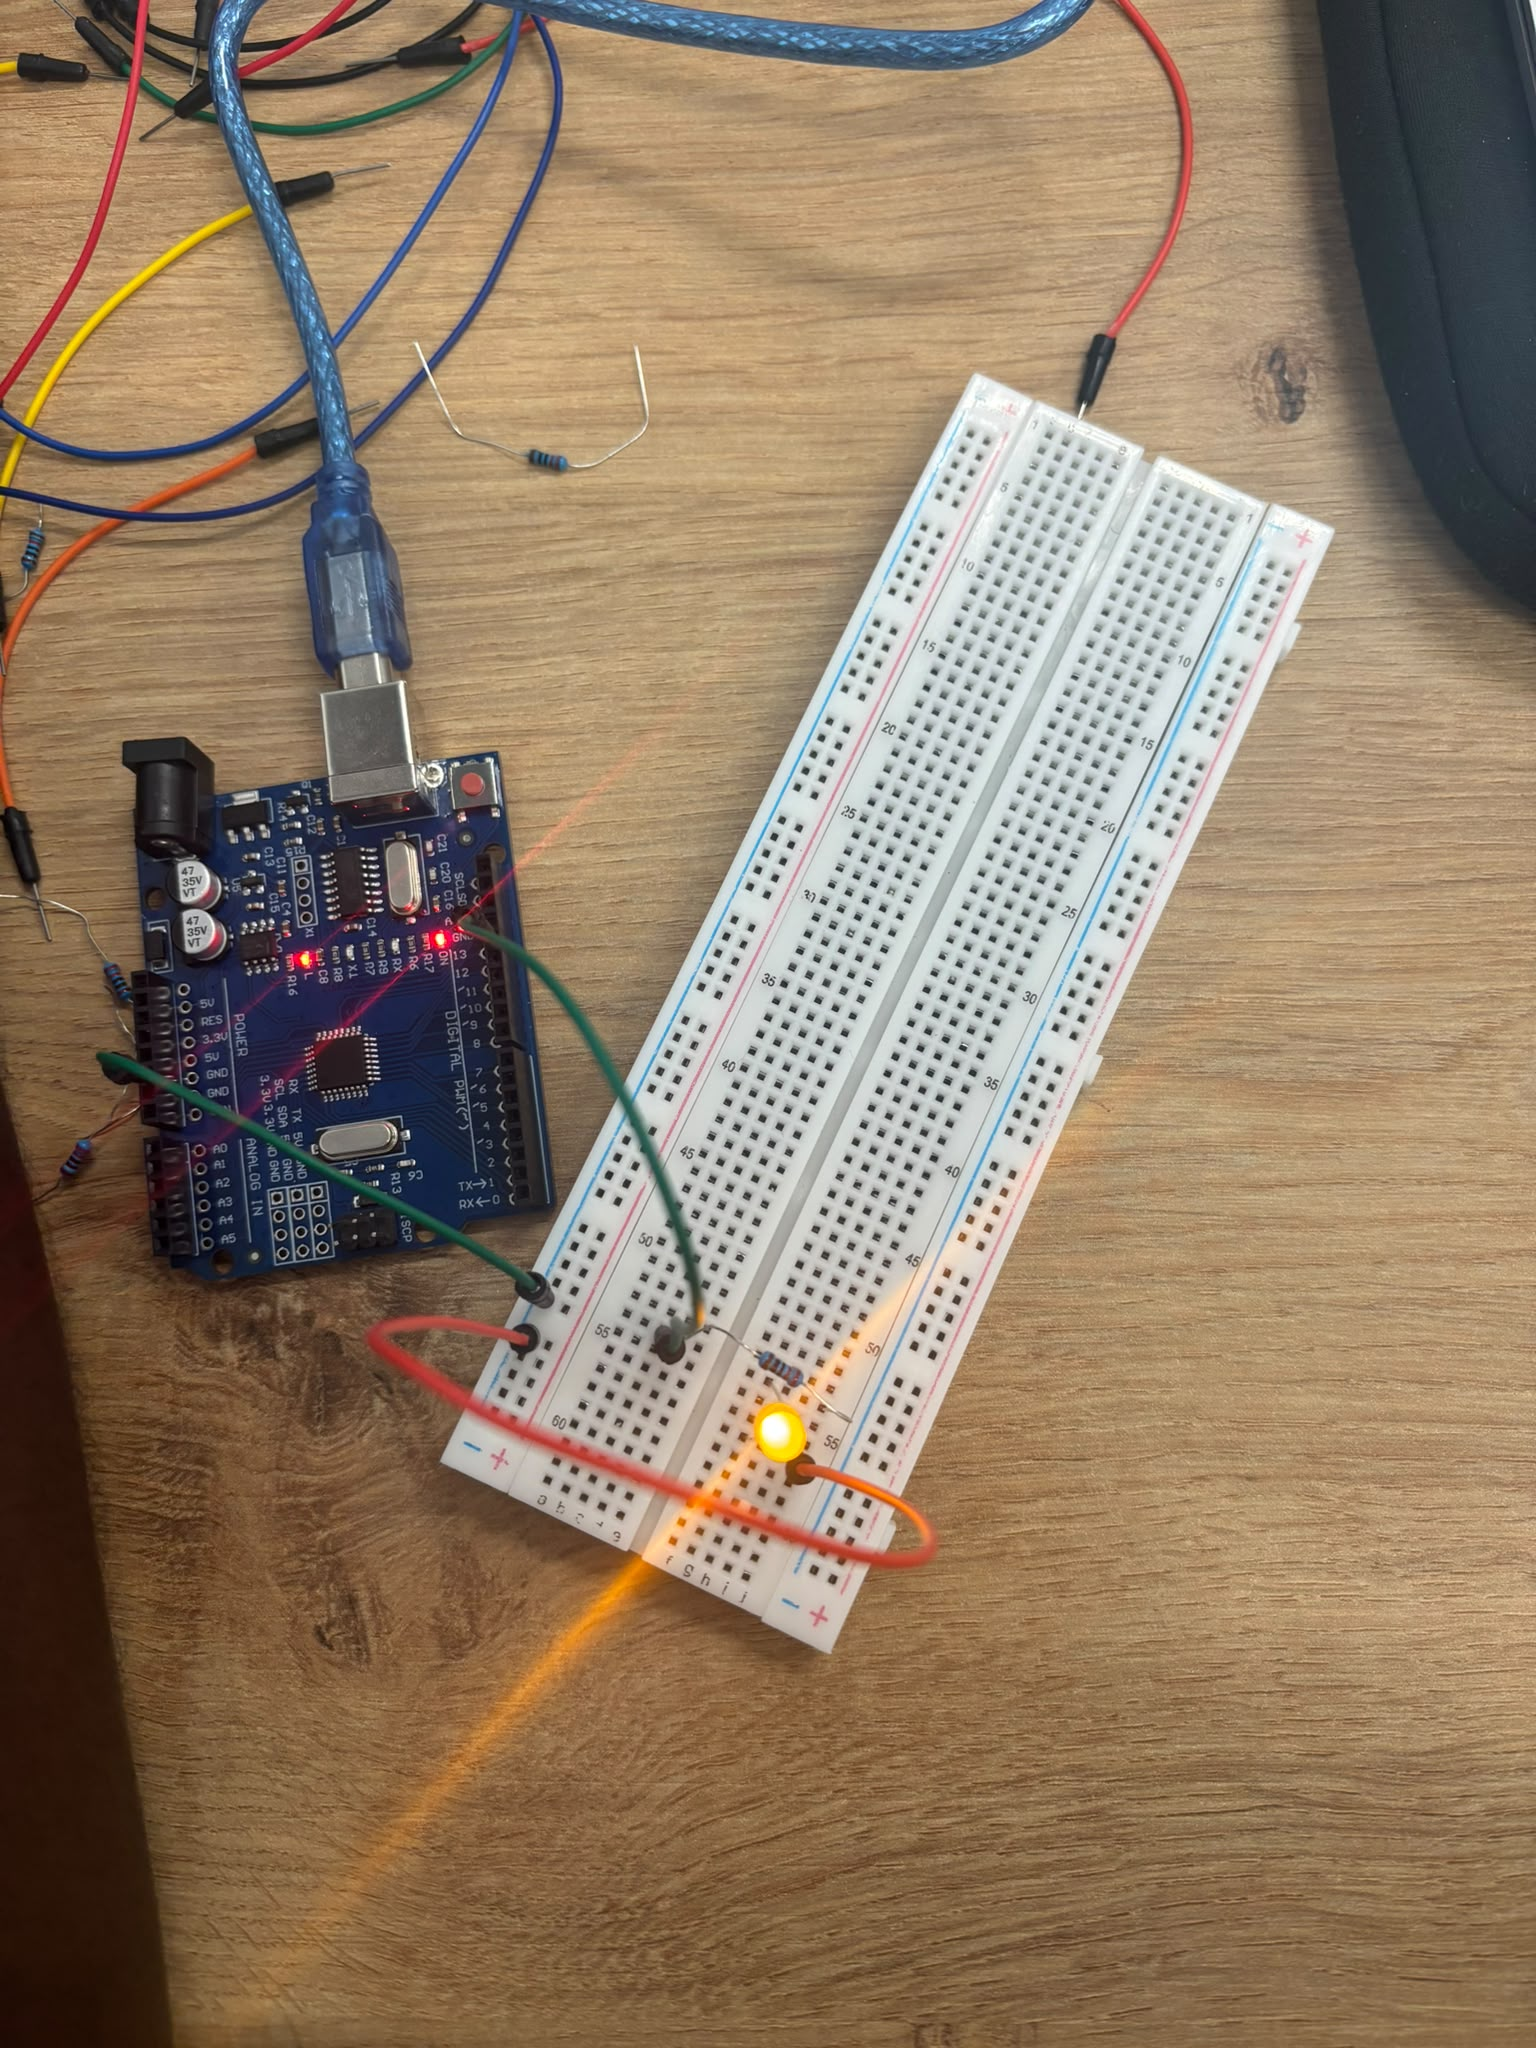
\includegraphics[width=0.7\linewidth]{Image/3.Resusltat}
	\caption{Led contrôlé a l'aide de Matlab}
	\label{fig:simulink_led}
\end{figure}	
\textbf{Observations :} La LED s'allume bien avec le code Matlab.

\paragraph{e) Commande d'un servomoteur avec MATLAB/Simulink}
De la même manière, nous contrôlons la position angulaire d'un servomoteur à d'un script Matlab.

\begin{lstlisting}
	clear a;
	clear s;
	a = arduino('/dev/ttyUSB0', 'Uno');
	s = servo(a, 'D9'); 
	angle = input('Entrez langle souhaite (entre 0 et 180) : ');
	writePosition(s, angle / 180);
\end{lstlisting}
\begin{figure}[H]
	\centering
	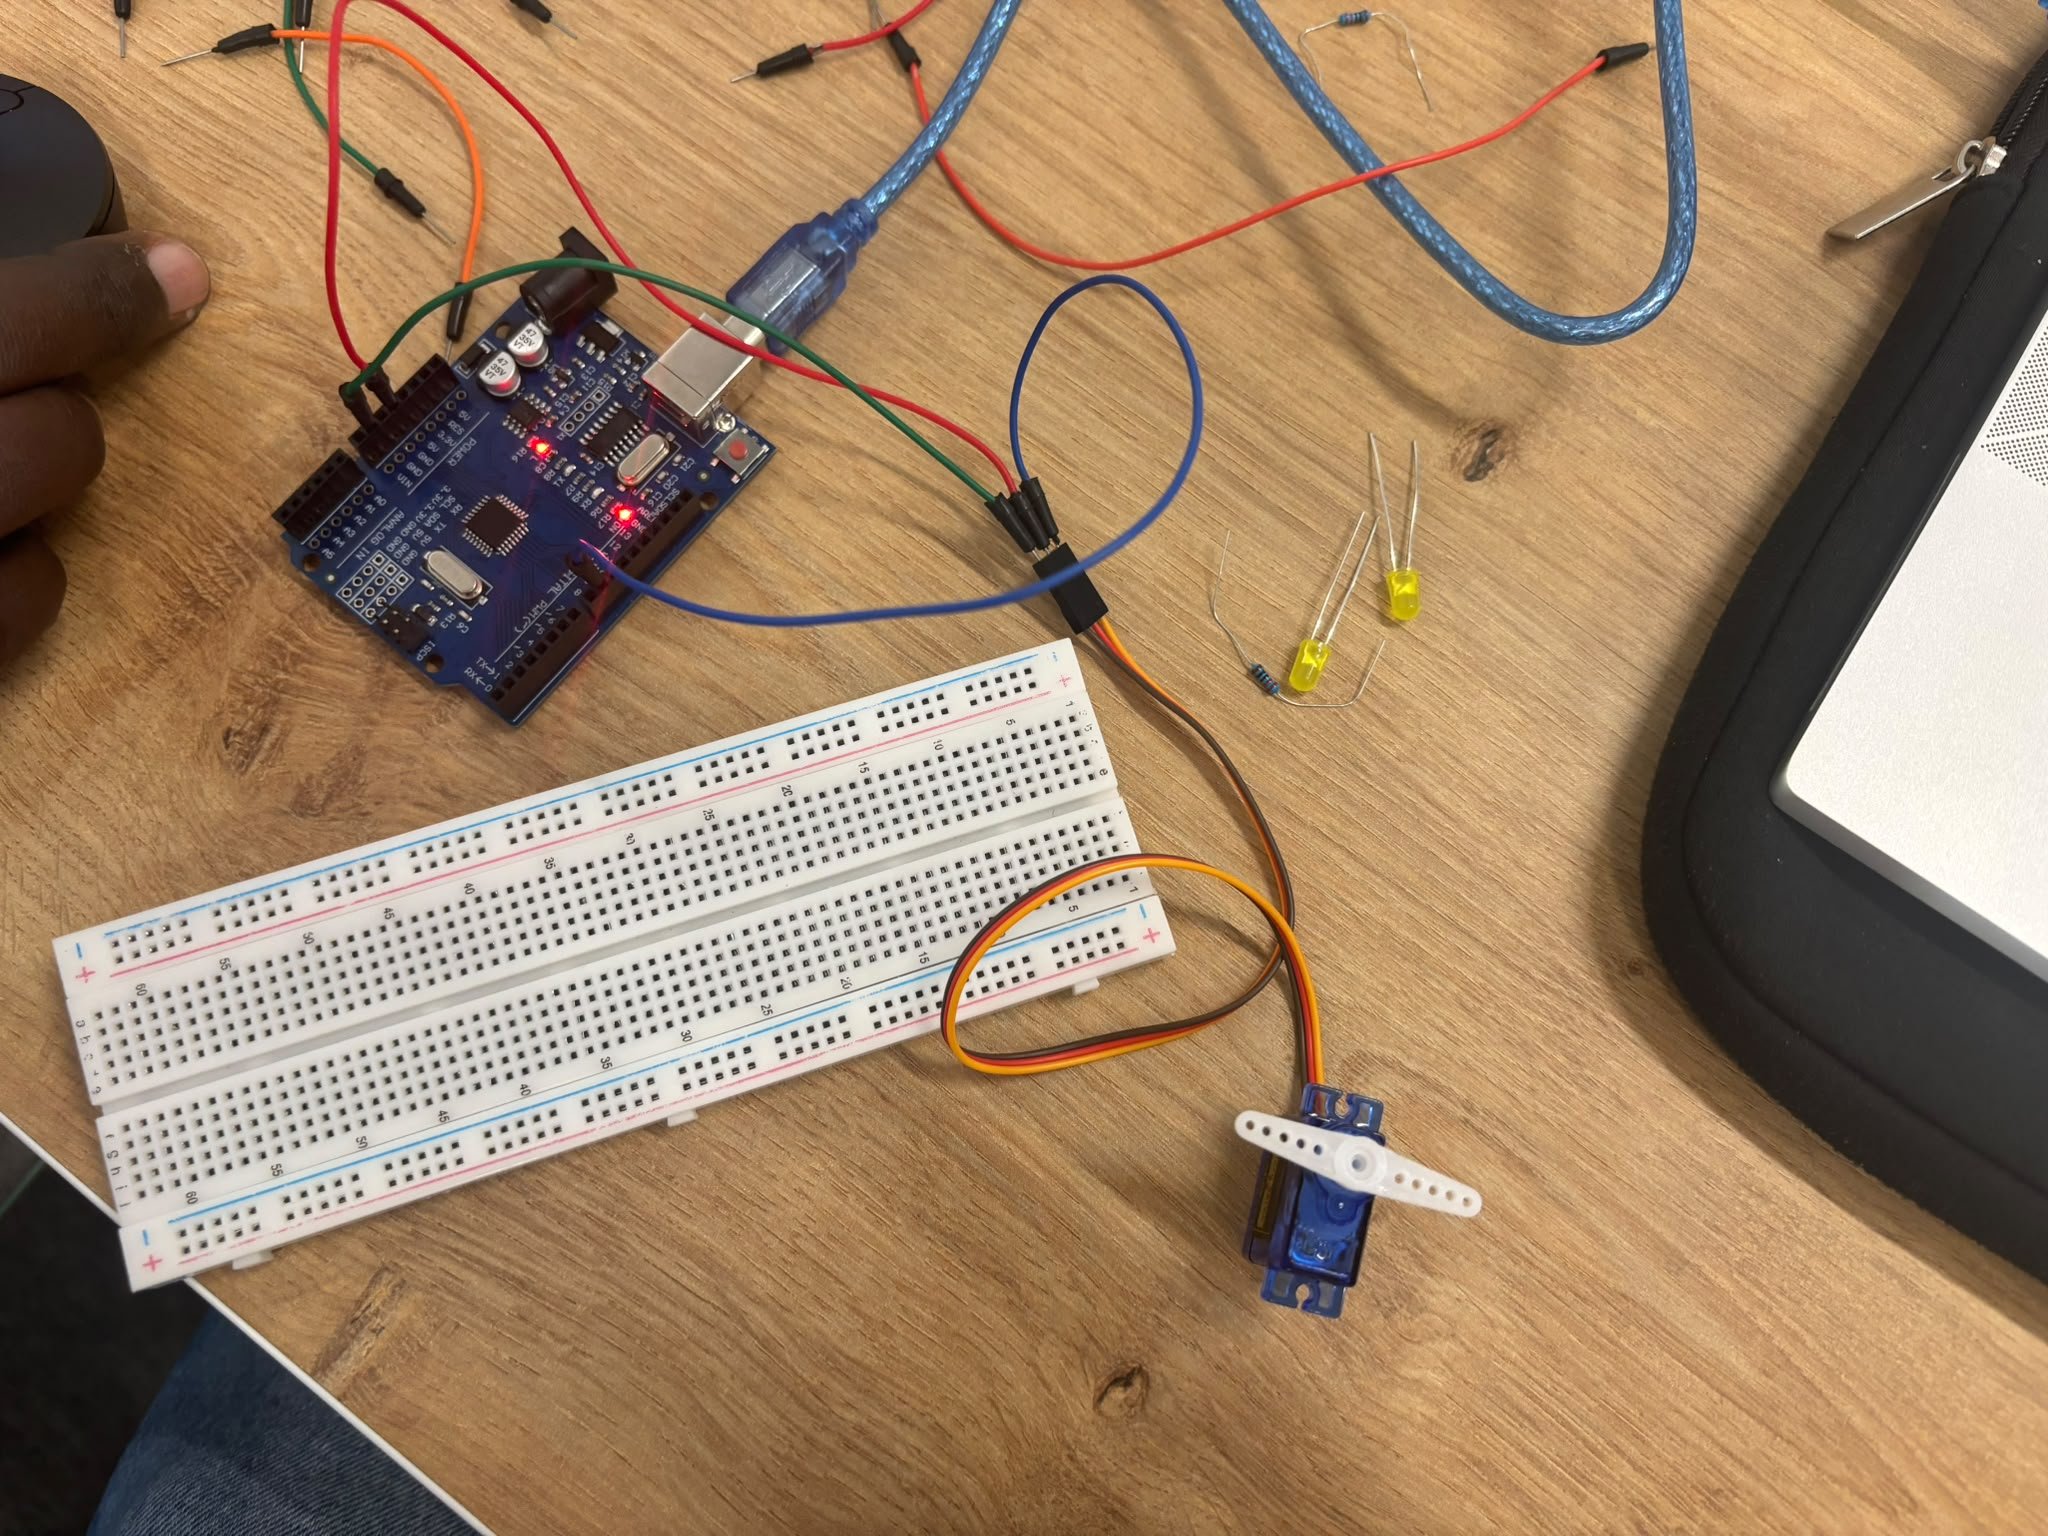
\includegraphics[width=0.7\linewidth]{Image/3.Servo}
	\caption{Servomoteur contrôlé a l'aide de Matlab}
	\label{fig:simulink_led}
\end{figure}
\textbf{Observations :} Le moteur change de position en fonction de l'angle que nous lui donnons avec notre code.

\section{Asservissement en vitesse d'un moteur avec régulateur PID}
\paragraph{f) Composants et schéma pour l'asservissement}
Pour cette dernière partie, nous devons mettre en place un système complet d'asservissement en vitesse en utilisant un régulateur PID modélisé sous MATLAB/Simulink et implémenté sur Arduino.

\textbf{Composants nécessaires :}
\begin{itemize}
	\item Carte Arduino Uno
	\item Moteur à courant continu (CC)
	\item Pont en H (Hacheur, ex: L298N) pour la partie puissance
	\item Capteur de Vitesse
	\item Alimentation externe pour le moteur
\end{itemize}

\begin{figure}[H]
	\centering
	 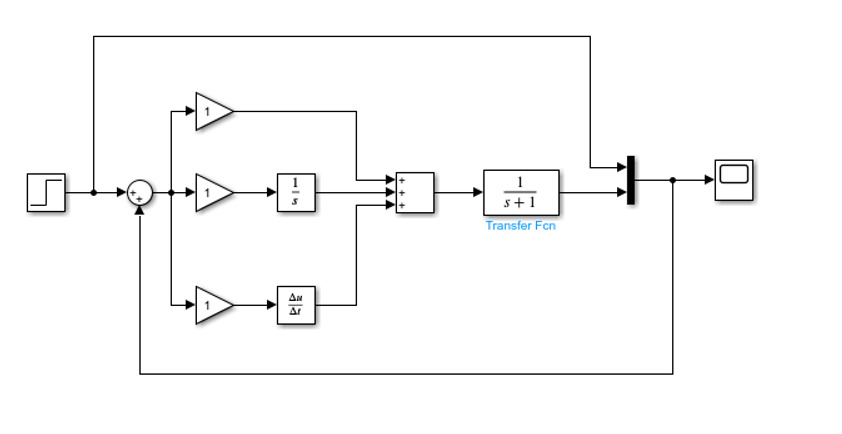
\includegraphics[width=0.8\linewidth]{Image/3.Schema_Asservissement}
	\caption{Modèle Simulink du régulateur PID}
	\label{fig:pid_moteur}
\end{figure}
